\section{Contrôles de la caméra}
L'application a pour but d'être utilisé sur mobile et tablette mais cela n'empêche pas qu'elle soit accessible par un ordinateur. Cela implique qu'il faudra gérer de manière différente ces deux types de clients. Afin de détecter à quel type d'appareil la page doit répondre, la meilleure technique est encore d'utiliser une expression régulière sur le \emph{User agent} \cite{wiki-useragent}.

\subsection{Orientation mobile}
Sur un ordinateur il est possible de se déplacer à l'aide des touches fléchées, sur un mobile on ne peut pas utiliser le même fonctionnement. L'idée est d'utiliser le gyroscope interne du smartphone à l'aide de l'API \emph{DeviceOrientation \& DeviceMotion events}\cite{w3c-orientation} supporté par tous les navigateurs mobile\cite{caniuse-DeviceMotion}. 

Le senseur nous envoie alpha, beta et gamma qui sont respectivement les rotations sur les axes Z, X' et Y'', voir Figure \ref{fig:mobile-angles}. On peut en déduire facilement les angles d'\emph{Euler}, puis il est possible d'en trouver le quaternion qui exprime la rotation que l'on applique ensuite à notre caméra. Cependant les smartphones n'envoient pas forcément des valeurs absolues, c'est à dire qu'il n'est pas possible de trouver le Nord à partir de ces valeurs. Le magnétomètre n'est pas accessible depuis une page web, ce qui aurait pu nous aider à trouver le Nord. L'interface utilisateur permet de décaler la valeur alpha du gyroscope à gauche ou à droite, afin de pouvoir calibrer à la main son orientation.

\begin{figure}
	\centering
	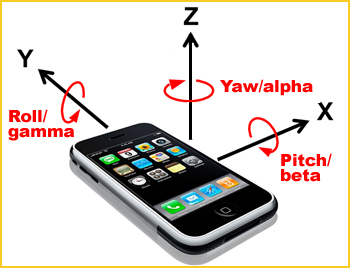
\includegraphics[width=0.4\linewidth]{mobile-sensors}
	\caption{Les axes ainsi que leurs rotations respectives d'un téléphone mobile. Source image: \url{http://hillcrestlabs.com}}
	\label{fig:mobile-angles}
\end{figure}

\subsection{Suivi du chemin}
Après que l'utilisateur ait choisi un point A et un point B, l'algorithme de recherche de chemin va définir un itinéraire à suivre. La caméra doit parcourir ce chemin tout en gardant une certaine orientation afin que l'utilisateur comprenne. Afin que les contours soit plus naturels et moins brutaux il est important d'interpoler les points que l'on doit suivre. Dans le cas d'Arc3D, c'est une interpolation avec méthode de Catmull-Rom qui est utilisé. Ceci pour la raison que cette méthode fonctionne avec autant de points que nécessaire et que c'est une méthode déjà connue de ma part.

Il réside encore un problème, si le mode \textit{à mobilité réduite} est activé la recherche de chemin va plutôt emprunter les ascenseurs que les escaliers. Dans ce cas là on va créer des courbes supplémentaires, pour chaque section du tracé, voir figure \ref{fig:spline-stairselevator}. Le programme calcule la distance parcourue de l'utilisateur est détermine sur laquelle des courbes il se trouve.

\begin{figure}
	\centering
	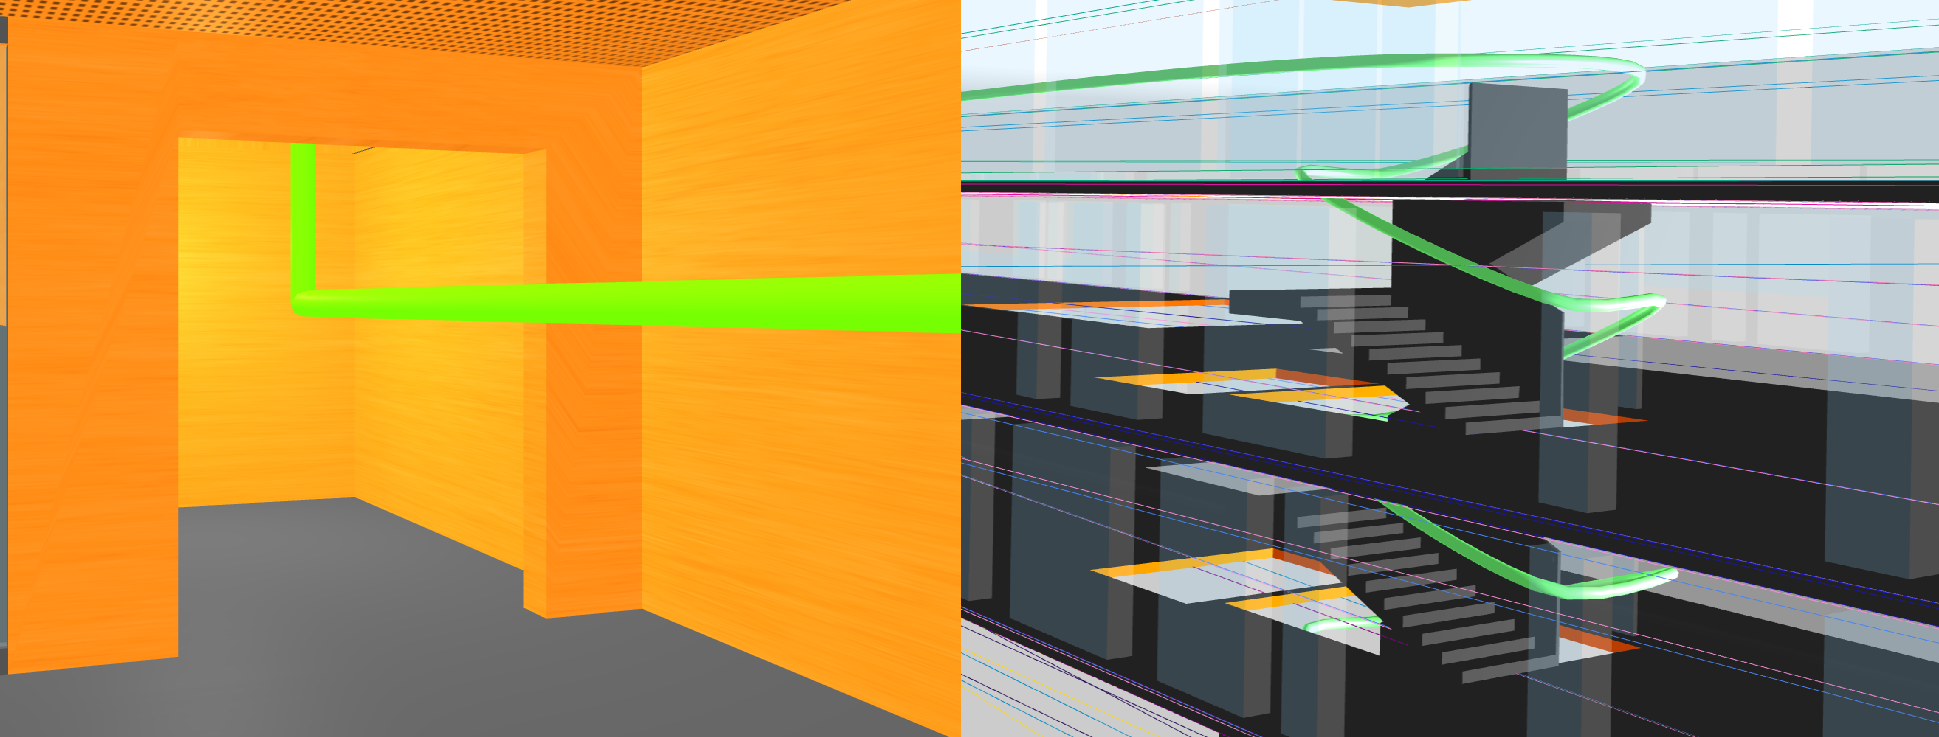
\includegraphics[width=0.9\linewidth]{spline-StairsElevator}
	\caption{La différence entre une courbe qui passe par les escaliers ou un ascenseur.}
	\label{fig:spline-stairselevator}
\end{figure}

Ensuite, il reste à définir la direction de la caméra. Comme expliqué avant, il y a une courbe pour chaque section du tracé. Chacune de ces dernières est lié à un comportement qui est différent pour les ascenseurs (\textit{elevator behaviour}) que pour les autres sections (\textit{normal behaviour}). Le comportement de type \emph{normal} va simplement regarder un point qui se trouve à une certaine distance sur la courbe. Tandis que le comportement \emph{elevator} est décrit comme suit: 
Au début d'une courbe \emph{elevator}, on stocke un vecteur unitaire dans la dernière direction de la courbe précédente et un deuxième dans la première direction de la courbe suivante. Ensuite, tout au long du trajet on effectue une interpolation linéaire entre les deux vecteurs directeurs calculés précédemment.

Ce qui permet d'imiter le comportement d'un humain dans un ascenseur. Ce dernier a généralement tendance à pivoter sur lui même pour être prêt à sortir du bon côté de l'ascenseur.

\subsubsection{Live et Simulation}
L'application propose encore deux modes de visualisation différents. Ces derniers ont été nommés \emph{Live} et \emph{Simulation}. Le mode \emph{Live} devait à la base représenter le mode où l'utilisateur était géolocalisé en permanence. Étant donné que cet objectif n'était pas réalisable c'est un autre mécanisme qui a été mis en place. La visualisation procède au déplacement seulement si l'orientation du téléphone regarde le chemin. Tandis que le mode \emph{Simulation} se déplace sans arrêt et la caméra est fixé sur le chemin.
